\chapter{Métodos e Desenvolvimento}
\label{cap:desen}
Este capítulo descreve as etapas de desenvolvimento e as metodologias empregadas neste trabalho. Buscaram-se estratégias sem intrusão ou grandes modificações nas políticas de escalonamento já implementadas pelo \textit{framework}. Nas Seções \ref{sec:collector} e \ref{sec:zookeeper} são apresentados em maior detalhe os coletores de contexto e a ferramenta de comunicação distribuída utilizados neste trabalho, respectivamente. Finalmente, na Seção \ref{sec:solucao} explica-se em profundidade a solução implementada neste trabalho e as justificativas para as decisões tomadas.

%-------------------------------------------------------------------
\section{Coletores de Contexto}
\label{sec:collector}
Após um estudo aprofundado dos escalonadores do Hadoop, ficou claro que o Capacity Scheduler já está estruturado de maneira a oferecer escalabilidade e um desempenho satisfatório. Porém, este escalonador possui um ponto fraco, o qual é exposto quando utilizado em um ambiente compartilhado. O Capacity Scheduler só recebe informações sobre os Node Managers no momento da inicialização destes, e ainda, a informação é obtida de um arquivo de configuração. A importância de que as informações sobre os Node Managers estejam atualizadas decorre da dependência intrínseca do escalonamento com a disponibilidade de recursos, na qual uma informação errada pode influenciar o algoritmo de maneira prejudicial e diminuir o desempenho das tarefas. Com base nestas observações, o primeiro passo para a solução é a coleta de dados sobre os recursos dos Node managers, ou seja, a adição de sensibilidade ao contexto.

\subsection{Sensibilidade ao Contexto}
\label{sec:ctx}
Contexto é definido por \cite{Dey} como qualquer informação que pode ser utilizada para caracterizar a situação de uma entidade (pessoa, lugar ou objeto) considerada relevante para a interação entre usuário e aplicação. Um exemplo de utilização de contexto é quando um usuário acessa um site por meio de um dispositivo móvel e o site carrega automaticamente a versão \textit{mobile}, a qual possui alterações que aumentam a compatibilidade com o tipo de dispositivo sendo utilizado. Outra situação semelhante ocorre quando dados de localidade são utilizados para melhorar os resultados de um motor de buscas, mostrando primeiro os resultados mais relacionados com a região ou idioma do usuário. Nota-se que nas duas situações a aplicação utiliza dados específicos, o tipo do dispositivo e a localização do usuário, coletados no momento da execução e utiliza-os para adaptar o seu funcionamento de maneira a oferecer maior conforto ou usabilidade ao usuário. 

Sendo assim, se uma aplicação é capaz de coletar informações sobre a situação do sistema no qual está sendo executada, ela é capaz de coletar informações de contexto. Porém a simples coleta não aumenta, de fato, o desempenho desta aplicação, é necessário que a aplicação seja capaz de responder às mudanças detectadas no ambiente. Esta capacidade de detecção e reação é caracterizada como sensibilidade ao contexto por \cite{Maamar} e vai ao encontro da definição de \cite{Baldauf} em que o sistema deve detectar mudanças e adaptar suas operações sem intervenção explícita do usuário, aumentando assim a usabilidade e eficácia da aplicação.

\subsection{Implementação}
Em um primeiro momento, buscou-se diminuir a dependência nos arquivos XML para a configuração dos recursos dos Node Managers com intuito de facilitar a configuração inicial dos nós e futuramente utilizar este mesmo mecanismo para a inclusão do suporte ao compartilhamento dos recursos. Para isto, fez-se necessário o desenvolvimento de um conjunto de coletores de contexto capazes de coletar de maneira eficiente os recursos do nó em questão no momento da inicialização do serviço Node Manager e, consequentemente, passar a informação correta sobre os recursos no momento do registro no Resource Manager.

Embora esta adição já facilite a utilização do Hadoop em um \textit{cluster} de natureza heterogênea, ainda não é suficiente para que o Hadoop seja utilizado eficientemente em um \textit{cluster} compartilhado. A razão para esta afirmação é que, embora a informação esteja correta no momento de inicialização, é possível que durante a execução das aplicações de \textit{MapReduce} os recursos comecem a ser utilizados por outros usuários, diminuindo a capacidade disponível para o Hadoop. O problema causado pela utilização de alguns nós por outros usuários sem a devida atualização dos dados no escalonador é a sobrecarga destes nós, uma vez que o Hadoop irá tentar utilizar memória e processadores que já estão alocados à outros processos.
% causando, nos piores casos, \textit{Swap} da memória.
%TODO Se deixar isso, colocar dados de swap nos testes

Com objetivo de solucionar o problema causado pelo compartilhamento, é necessário que a coleta de dados ocorra não apenas na inicialização do Node Manager mas ao longo da execução do serviço em intervalos periódicos. Para isso optou-se pela utilização de uma \textit{thread} para a coleta e transmissão, se necessária, dos dados.

O coletor escolhido para a tarefa foi o coletor desenvolvido pelo projeto PER-MARE \cite{Collector}, o qual utiliza a interface padrão do Java para monitoramento, OperatingSystemMXBean \cite{MXBean}. A implementação deste coletor de contexto é baseada em uma interface, uma classe abstrata e as classes de coleta dos recursos desejados. Devido ao seu projeto, coletores de novas informações podem ser facilmente criados, aumentando assim a quantidade de informação disponível para o escalonador.

A interface OperatingSystemMXBean, possibilita o acesso às informações do sistema no qual a JVM está sendo executada. Uma vez que a classe abstrata implementa esta interface, todas suas herdeiras poderão utilizá-la.

As classes utilizadas neste trabalho fazem a coleta de memória física disponível e processadores disponíveis, os recursos suportados por padrão no Hadoop. É possível visualizar o digrama de classes na figura \ref{fig:collectorUML}, onde estão presentes alguns exemplos de possíveis coletores a serem utilizados.

%TODO fazer outro DC
\begin{figure}[!hbtn]
   \centering
   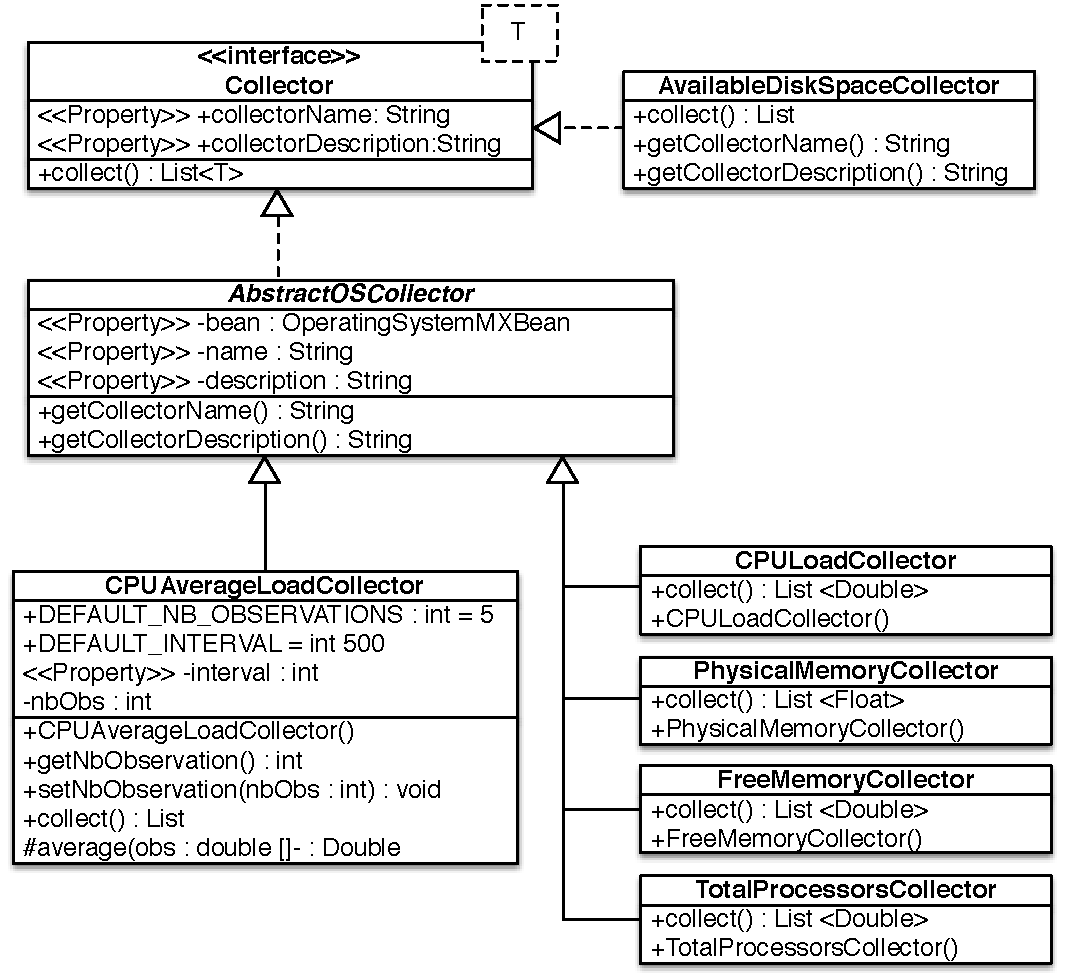
\includegraphics[width=15cm]{figuras/CollectorUML2.pdf}
   \caption{Diagrama de classes dos coletores de contexto}
   \label{fig:collectorUML}
\end{figure}

Cada instância de Node Manager possui um conjunto de coletores (um para memória e um para processadores), os quais realizam a coleta num intervalo pré-definido. Os coletores são executados por uma \textit{thread} independente e possuem um intervalo de 30 segundos entre as coletas para não causar sobrecarga ou interrupção no  processamento das tarefas \textit{Map} e \textit{Reduce}.

%-------------------------------------------------------------------
\section{Comunicação Distribuída}
\label{sec:zookeeper}

Para que a informação coletada pelos coletores de contexto possa afetar o escalonamento é necessário que exista uma maneira para os Node Managers transmitirem os dados atualizados ao escalonador, a ferramenta escolhida para esta tarefa foi o ZooKeeper.

\subsection{ZooKeeper}
O ZooKeeper é um projeto da Apache e fornece ferramentas eficientes, confiáveis e tolerantes à falha para a coordenação de sistemas distribuídos \cite{Hunt2010}. Inicialmente, o ZooKeeper foi implementado como um componente do Hadoop e virou um projeto próprio conforme cresciam suas funcionalidades e sua utilização em outras aplicações. 

A arquitetura utilizada no ZooKeeper é a de cliente-servidor, sendo o servidor o próprio ZooKeeper (chamado de \textit{ensamble}), enquanto a aplicação que o está utilizando assume o papel de cliente. Os dados do ZooKeeper ficam armazenados em \textit{zNodes}, abstrações que podem ser tanto um \textit{container} de dados quanto de outros \textit{zNodes}, e formam um sistema de arquivos hierárquico que pode ser comparado à estrutura de uma árvore. Para garantir a consistência deste sistema de arquivos o ZooKeeper utiliza operações de escrita linearizáveis, as quais são obrigatoriamente processadas pelo servidor líder que é, então, encarregado de propagar as mudanças para os demais participantes do \textit{ensamble} \cite{Pham}.

Um dos principais recursos do ZooKeeper são os \textit{Watchers}, interfaces providas pelo \textit{framework} que permitem aos clientes monitorarem certos \textit{zNodes}. Quando um \textit{Watcher} é registrado como monitor de um \textit{zNode}, ele pode ser configurado para monitorar a alteração dos dados do \textit{zNode}, a criação/remoção de \textit{zNodes} filhos, ou ainda para qualquer tipo de alteração no \textit{zNode} e seus filhos. Quando um \textit{zNode} sofre uma alteração que o \textit{Watcher} está monitorando uma \textit{callback} é disparada para que o cliente faça o processamento desejado. O disparo desta \textit{callback} é um evento único, forçando o programador a re-inserir um \textit{Watcher} no \textit{zNode} para continuar monitorando-o \cite{HadoopBook}.

No âmbito deste trabalho, os serviços do ZooKeeper são utilizados para monitorar as informações de contexto coletadas nos nós escravos e transmiti-las para o escalonador. Sendo que a comunicação é feita através de processos que atualizam e monitoram o conteúdo de \textit{zNodes}.

%----------------------
\subsection{Implementação}
A flexibilidade oferecida através dos \textit{zNodes} permite que qualquer estrutura de dado seja inserida como informação, porém existem alguns detalhes importantes no gerenciamento de \textit{Watchers} que podem impactar na eficácia da solução. Por esta razão optou-se por utilizar um \textit{zNode} para cada NodeManager, o que permite realizar um controle mais rígido das atualizações e possibilita uma maneira fácil e rápida tanto para a inserção das informações por parte dos Node Managers quanto para o monitoramento dos dados pelo escalonador.

Na solução adotada cada \textit{zNode} contém informação de apenas um Node Manager e para cada \textit{zNode} existe um Watcher, sendo que cada \textit{Watcher} é uma thread pertencente ao escalonador. Qualquer alteração em um \textit{zNode} dispara uma \textit{callback} para seu \textit{Watcher} específico, o qual lê os novos dados do \textit{zNode} e atualiza a informação no escalonador sobre os recursos daquele nó. A utilização do \textit{Watcher} permite que o escalonador realize operações apenas quando necessário e não desperdice tempo percorrendo os \textit{zNodes} quando não houverem atualizações a serem feitas. A estrutura adotada no trabalho podes ser visualizada na Figura \ref{fig:zk}.


%Qualquer alteração na tabela dispara uma \textit{callback} no escalonador, que por sua vez percorre a tabela à procura das modificações e realiza as alterações pertinentes nas informações sobre os recursos. Esta abordagem permite que o escalonador realize operações apenas quando necessário e não desperdice tempo acessando a tabela quando não houverem atualizações a fazer. A estrutura adotada no trabalho podes ser visualizada na Figura \ref{fig:zk}.


\begin{figure}[!hbtn]
   \centering
   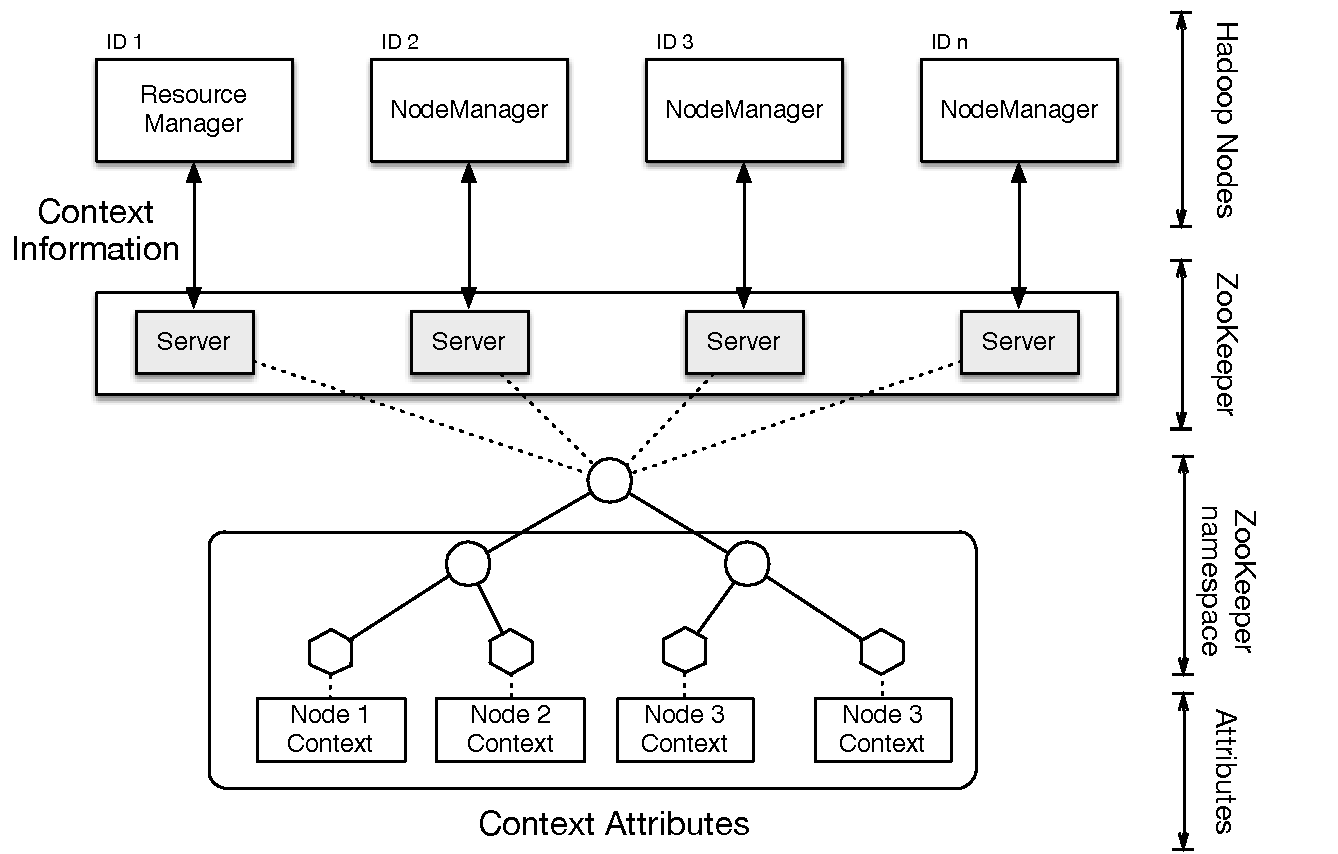
\includegraphics[width=15cm]{figuras/Zookeeper.pdf}
   \caption{Estrutura do ZooKeeper}
   \label{fig:zk}
\end{figure}

A solução escolhida gera dois papéis para os nós, o papel de monitoramento e o papel de atualização, os quais são explicados em detalhe a seguir.

O papel de \textbf{Monitoramento} é desempenhado pelo escalonador, o qual possui uma \textit{thread} \textit{Watcher} que monitora um \textit{zNode}. Este \textit{zNode} inicial servirá como \textit{container} para os demais \textit{zNodes}, os quais armazenarão as informações de contexto referentes aos nós escravos do \textit{cluster}. O \textit{Watcher} do \textit{zNode} inicial permite ao escalonador ser notificado quando novos \textit{zNodes} forem inseridos na estrutura. Quando a \textit{callback} do \textit{Watcher} é acionada, a \textit{thread} recebe todos os \textit{zNodes} filhos daquele que está sendo monitorado e após identificar o novo \textit{zNode}, inicia uma nova \textit{thread Watcher} para monitorar o novo \textit{zNode} identificado. Desta forma, cada \textit{zNode} será monitorado por uma \textit{thread Watcher} única. Um possível problema da técnica utilizada é discutido, juntamente com a solução adotada para solucioná-lo, na descrição do papel de Atualização.

Uma alternativa à utilização de um \textit{zNode} para cada nó escravo, seria a utilização de uma estrutura que permitisse a inserção de todos os dados dos nós escravos, como uma Tabela Hash. Embora em um primeiro momento o maior impecilho para a utilização desta técnica possa parecer o limite padrão do tamanho da informação que um \textit{zNode} comporta (1 Mb), o problema é, na verdade, relacionado com a utilização de uma única \textit{thread Watcher}. 

Como todos os nós escravos são, geralmente, inicializados ao mesmo tempo, as coletas de dado são realizadas em períodos semelhantes, esses períodos serão denominados neste estudo como fase de coleta. Durante estas fases, é possível que muitas atualizações sejam feitas em um pequeno espaço de tempo, gerando um risco à consistência das informações, uma vez que o ZooKeeper não fornece garantias de que todas as alterações notificarão a \textit{thread Watcher}. Este comportamento ocorre devido à possibilidade de notificações serem disparadas antes da re-inserção do \textit{Watcher} no \textit{zNode} que contém a Tabela Hash. Esta falha só ocorre quando a segunda notificação é enviada antes que a primeira termine de ser processada, e existem duas situações que isto pode ocorrer. A primeira situação não apresenta grandes riscos à consistência das informações, pois a notificação perdida  ocorre entre duas notificações normais na mesma fase de coleta. Sendo assim, a notificação seguinte fará com que o escalonador ajuste os valores de recursos dos dois nós. Já a segunda situação apresenta riscos à consistência das informações, pois ocorre quando não há uma notificação normal na mesma fase de coleta após a notificação perdida, ou seja, a notificação perdida só terá suas informações atualizadas no escalonador na próxima fase de coleta, a qual ocorrerá em aproximadamente 30 segundos. Este período que o escalonador opera com informações inconsistentes pode causar o lançamento de \textit{containers} que irão exceder o limite dos nós caso um novo usuário tenha iniciado a utilização do nó, gerando sobrecarga e lentidão tanto na aplicação do novo usuário como na aplicação MapReduce.

%	o papel de monitor é desempenhado pelo escalonador. O escalonador implementa a interface Watcher, fornecida pelo ZooKeeper, e monitora o \textit{zNode} que contém a Tabela Hash. No momento da inicialização o escalonador cria um \textit{zNode} e insere uma Tabela Hash vazia como informação, então finalmente, inicia o monitoramento do \textit{zNode}. Quando a \textit{callback} é acionada, a \textit{thread} percorre a tabela em busca de qual informação foi atualizada, atualiza os dados do escalonador e reinicia o monitoramento.
	
O papel de \textbf{Atualização} é realizado pelos Node Managers, os quais lançam, no momento de sua inicialização, uma \textit{thread} responsável por fazer a coleta de dados e, caso houver alteração com relação à ultima coleta, atualizar os dados no \textit{zNode}. A coleta dos dados é realizada a cada 30 segundos, intervalo que corresponde à média de tempo observada em \textit{containers} executados em um \textit{cluster} de funcionamento normal. Com objetivo de evitar o envio de dados por alterações naturais do sistema e que não impactariam no escalonamento foi implementada uma política de atualização, na qual atualizações só serão realizadas quando as variações alterarem o limite de \textit{containers} que podem ser inicializados no nó, seja pela carga de CPU ou disponibilidade de memória. Esta política permite ao escalonador otimizar seu poder de adaptabilidade sem desperdiçar tempo com leituras desnecessárias ou transmissão de dados não diretamente relacionados com as aplicações.

Ao evitar a atualização por variações que não impactem na capacidade de \textit{containers}, a quantidade de dados transmitidos é reduzida e, consequentemente, o número de execuções das \textit{threads} \textit{Watcher} que monitoram os \textit{zNodes} também o são. Caso esta política não fosse utilizada, correria-se o risco de todos os nós escravos apresentarem variações em todas as leituras. Sabe-se que o sistema operacional possui alterações naturais dos recursos e que estas, geralmente, não representam uma grande quantidade de recursos. Além disso, segundo a política de alocação de \textit{containers} do Hadoop e utilizando os valores \textit{default}, tanto um nó com 1024 Mb livres quanto um nó com 2047 Mb livres serão capazes de inicializar somente 1 \textit{container} \cite{tg}. Por este motivo, a atualização de variações que não alterem a quantidade máxima de \textit{containers} em um nó somente desperdiçariam tráfego na rede e processamento nos nós. Em um cluster de 100 nós, por exemplo, este comportamento poderia causar a execução de 100 \textit{threads} no nó mestre a cada 30 segundos, sem levar em consideração a transmissão de dados pela rede. Contudo, uma vez que a variação representa uma alteração na capacidade de \textit{containers} do nó, a atualização deve ser feita. Caso a variação seja positiva (mais \textit{containers} podem ser lançados), a não atualização impactaria no desperdício de capacidade que ficaria ociosa. No caso da variação ser negativa (menos \textit{containers} podem ser lançados), a não atualização faria o escalonador ignorar a sobrecarga e continuar lançando novos \textit{containers} mesmo que estes estivessem acima da capacidade do nó.

%-------------------------------------------------------------------
\section{Solução Implementada}
\label{sec:solucao}
Estudos prévios indicam que o Capacity Scheduler já apresenta uma boa base para introdução de sensibilidade ao contexto e adaptatividade no Hadoop \cite{tg}. Uma vez que o objetivo deste estudo foi melhorar a adaptabilidade à ambientes com presença de compartilhamento, um dos principais mecanismos necessários foi o de adaptação à fatores que sofrem alterações no decorrer do processamento de tarefas. Assim, foi implementada uma nova funcionalidade no escalonador que permite a ele adaptar-se às variações de recursos disponíveis nos nós durante a execução de aplicações MapReduce. A solução implementada utiliza tanto os coletores de contexto quanto a comunicação distribuída por meio do ZooKeeper.

Como já citado anteriormente, o custo de aquisição e manutenção de um \textit{cluster} dedicado para a execução de aplicações MapReduce é alto e é possível que pequenas empresas, que não tenham recursos financeiros suficientes para a aquisição de um \textit{cluster}, prestem serviços que geram uma grande quantidade de dados. Embora estes casos possam ser resolvidos com a utilização de \textit{IaaS} (Infrastructure as a Service -- Infra-estrutura como Serviço) como o Amazon AWS \cite{amazonAWS} e Amazon EC2\cite{amazonEC2} a custos baixos, os proprietários podem preferir não utilizar serviços em nuvem devido à outros fatores como a segurança de dados pessoais ou adaptação à nova tecnologia. Nestes casos a utilização da capacidade ociosa dos computadores na rede da empresa pode ser uma alternativa viável, uma vez que não gera custos de aquisição e a manutenção é mais simples.

O problema da utilização do Hadoop nestas condições é que, embora em menor escala, esta alternativa reproduz muitas das características presentes em \textit{grids} pervasivos, as quais podem impactar negativamente o desempenho do Hadoop. Dentro de um contexto de disponibilidade de recursos, é possível identificar 5 situações que podem ocorrer: a saída de um nó do \textit{cluster}, a entrada de um nó no \textit{cluster}, um nó que estava sendo utilizado pelo Hadoop passa a ser utilizado em conjunto para outra aplicação (início do compartilhamento), um nó que estava sendo compartilhado volta a ser totalmente disponível para o Hadoop (fim do compartilhamento) e os computadores podem ter configurações diferentes entre si (nós heterogêneos).

A situação mais fácil de ser resolvida é a de nós heterogêneos, pois, mesmo sem alterações no comportamento do Hadoop, bastaria alterar os arquivos XML de configuração dos nós. No caso de não alteração dos arquivos XML, alguns nós poderiam ser sobrecarregados enquanto outros poderiam ser sub-utilizados. Contudo, com a solução proposta neste estudo, a disponibilidade de recursos é coletada e enviada ao escalonador. Com isso a informação estará sempre consistente com a realidade, e haverá um ganho de desempenho através da diminuição da sobrecarga e da sub-utilização.

A saída de um nó do \textit{cluster} já está coberta de maneira eficiente pelos procedimentos de tolerância a falhas do Hadoop. As tarefas que estavam sendo processadas pelo nó serão perdidas e terão que ser reiniciadas em outro nó. Além disso o \textit{pool} de recursos totais é reduzido de acordo com o tamanho do NodeManager.

A entrada (registro) de um novo nó necessita de mais etapas, contudo é possível de ser feita mesmo com a distribuição \textit{default} do Hadoop. É necessário que o \textit{host} do novo nó seja incluído no arquivo de configuração \textit{slaves} do mestre antes de ser inicializado o NodeManager no nó escravo. Uma vez que estas duas etapas estejam completas, o escalonador irá aumentar o \textit{pool} de recursos totais de acordo com a capacidade do novo nó ou 8 Gb de memória e 8 \textit{cores} na distribuição \textit{default}.

As duas situações restantes são mais interessantes, pois não há suporte para elas na distribuição \textit{default} do Hadoop. Esta capacidade de adaptação não seria necessária, uma vez que, desde seu projeto, todos os computadores que compõem o \textit{cluster} são considerados dedicados para uso do Hadoop. Ainda assim, haveria uma alternativa para a utilização compartilhada dos recursos com a distribuição \textit{default} do Hadoop. Esta alternativa seria mediante a configuração dos arquivos XML, ao configurar cada computador do \textit{cluster} com menos recursos do que os totais que ele possui. Esta alternativa, embora simples, não é eficiente, pois implica que ou a parcela não utilizada pelo Hadoop (a diferença entre o valor no arquivo XML e o valor real dos recursos) é constante, ou que haverão momentos tanto de sobrecarga como de sub-utilização do \textit{cluster}. Como já mencionado na Seção \ref{sec:zookeeper} Outra alternativa, também ineficiente, seria inicializar o \textit{cluster} com a capacidade ociosa de cada computador naquele momento configurada nos arquivos XML, executar uma aplicação MapReduce e em seguida terminar a execução dos serviços do Hadoop. Esta alternativa também está sujeita a alterações na disponibilidade de recursos e possível sobrecarga e/ou sub-utilização.

No caso de início de compartilhamento, o escalonador continua inicializando novos \textit{containers} mesmo que a capacidade do nó tenha sido excedida, causando sobrecarga e lentidão para o término das tarefas e, consequentemente, da aplicação. Com a contribuição deste estudo os recursos disponíveis para utilização pelo Hadoop no nó em questão serão reduzidos, porém nenhum \textit{container} já inicializado será preemptado. Ainda assim, a contribuição permite ao escalonador saber que determinado nó está sobrecarregado e, com base nesta informação, não alocar novos \textit{containers} neste nó até que a situação dos recursos esteja normalizada, ou seja, existirem recursos disponíveis capazes de alocar ao menos 1 \textit{container}.

No caso de término do compartilhamento a distribuição \textit{default}, quando configurada para um \textit{cluster} dedicado, terá o mesmo comportamento da solução implementada por este estudo. Como o escalonador nunca alterou a informação do nó, ao terminar o compartilhamento este nó voltará à situação inicial, a qual todo recurso do nó está disponível para o Hadoop. Nesta situação a abordagem \textit{default} do Hadoop, quando configurada para um \textit{cluster} dedicado é eficiente. No caso da solução implementada neste estudo, o nó fará a coleta, atualizará a informação no \textit{zNode} e o escalonador atualizará a capacidade do nó quando for notificado da alteração, porém haverá um atraso de no máximo 30 segundos para que as informações fiquem consistentes com relação à distribuição \textit{default}. No caso de utilização da distribuição \textit{default} configurada para utilizar somente uma parte de alguns nós estes recursos ficarão ociosos, piorando o desempenho por não utilizar todos os recursos disponíveis.